%!TEX root = ../main.tex

\section{Compton spectrum}
\label{sec:compton-spectrum}

Without knowing anything about the distribution of energies or deflection angles of
the scattered electrons, by examining \autoref{eq:electron-energy} it can already be
established that the energy the electron gains from the interaction is directly
proportional to $\left(1-\cos\theta\right)$, or in other words, by how much the
photon is scattered away from its original path. It follows that for \\
$\theta\,=\,$\SI{180}{\degree} the electron gains a maximum energy of

\begin{equation}
\label{eq:maximal-energy}
E_\text{max}=\frac{E_\gamma}{1+\frac{m_e c^2}{E_\gamma}}.
\end{equation}

Since the photon physically cannot dump more energy by this process, a sharp drop in
the Compton spectrum at $E_\text{max}$ is expected. This characteristic drop-off is
commonly called the \textbf{Compton edge}. Energetically lower than this cutoff lays
the \textbf{Compton continuum}. Over a wide range of energies that correspond to 
scattering angles $\theta\in[\SI{0}{\degree},\SI{180}{\degree}]$ the flux of 
electrons remains approximately constant. This follows directly from 
\autoref{eq:klein-nishina}. While the Compton continuum is symmetric in the idealised
spectrum given in \autoref{fig:compton-spectrum}, this is only really valid in the 
low energy limit. For higher photon energies forward scattering becomes much more
probable. An example of this is given in \autoref{sec:differential-cross-section}. 
The backscattering on the surrounding environment can also create a small peak in the spectrum.

\begin{figure}
	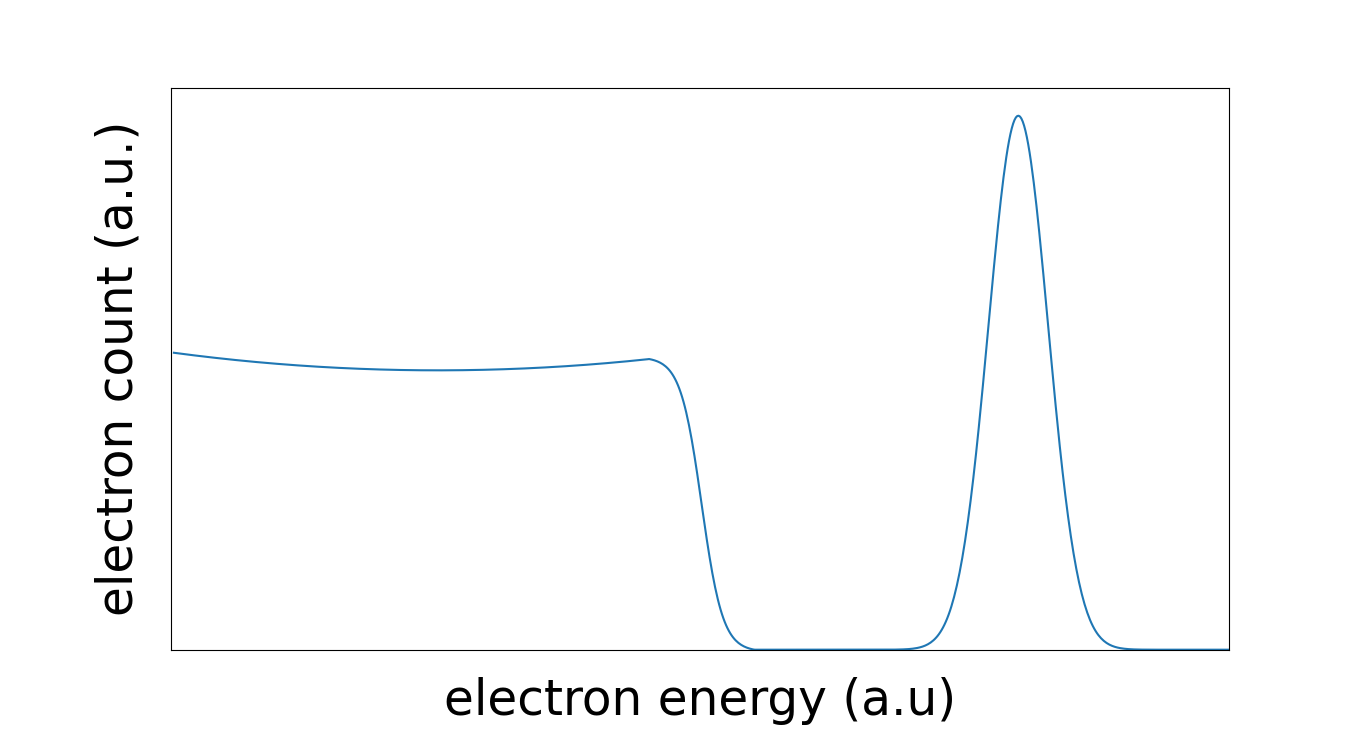
\includegraphics[width=1.0\textwidth]{fig/compton-spectrum}
	\caption{An idealised Compton spectrum. A relatively constant flux of
	electrons is measured up to an energy of $E_\text{max}$, where the spectrum
	sharply drops off, the so called \textbf{Compton edge}. At the high-energy end of the spectrum a gaussian shaped
	photopeak is visible.}
	\label{fig:compton-spectrum}
\end{figure}

Lastly, an idealised Compton spectrum will also display a characteristic 
\textbf{photopeak}. This photopeak is caused by photons directly interacting with 
detector material via the photoelectric effect. In this case, the entire energy of 
the photon (which is generally known a priori) is transfered to an photo-electron and then read out with the detector. It is 
therefore a helpful reference point for calibrations, albeit not being part of the 
Compton spectrum itself.

The measured Compton spectrum discussed in \autoref{chap:experiment} may display
several other characteristics such as a prominent X-ray line or a backscatter peak.
These properties are dependant on the experimental setup. As such they will -
if needed - be discussed in the appropriate sections of \autoref{chap:experiment}.
